\section{Estimator sweep and artifact round trip}
\label{sec:sweep}

The registry names 69 entries: 33 regression, 24 classification and 12 clustering. The sweep (\code{scripts/every\_model\_sweep.py}, record \code{docs/every\_model\_sweep\_2026-09-24.json}) trains each entry on a matching example dataset through the same function the web route calls, with the hyperparameters an empty form submits, so it exercises the path a user takes rather than a test harness of its own. Sixty-seven entries train; \code{Polynomial} (regression) and \code{Perceptron} (classification) are registered without a train function and are skipped, which is the state the registry is in rather than a failure of the two estimators. The whole sweep takes 49 minutes on the container's two cores; four estimators account for most of it (Figure~\ref{fig:seconds}): SVM regression at 385 seconds, RadiusNeighbors at 348, NuSVR at 291 and HistGradientBoosting at 240, all on the 442-row diabetes file with default settings and no search.

\begin{figure}[htbp]
\centering
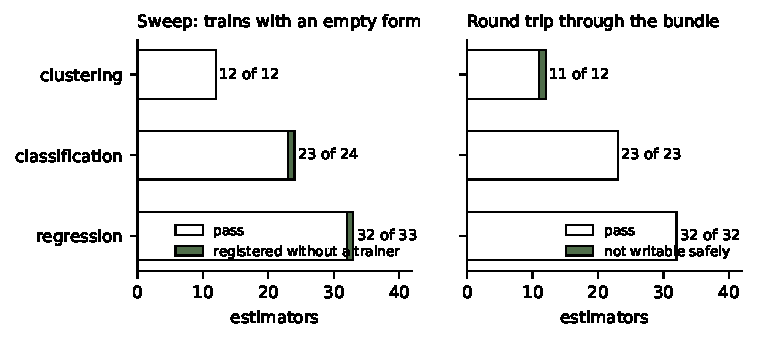
\includegraphics[width=0.75\textwidth]{fig_sweep_roundtrip}
\caption{Left: estimators that train with an empty form, by task. Right: estimators whose predictions are identical after a write to the bundle format and a read back. Sources: \code{every\_model\_sweep\_2026-09-24.json}, \code{artifact\_roundtrip\_2026-09-24.json}.}
\label{fig:sweep}
\end{figure}

\begin{figure}[htbp]
\centering
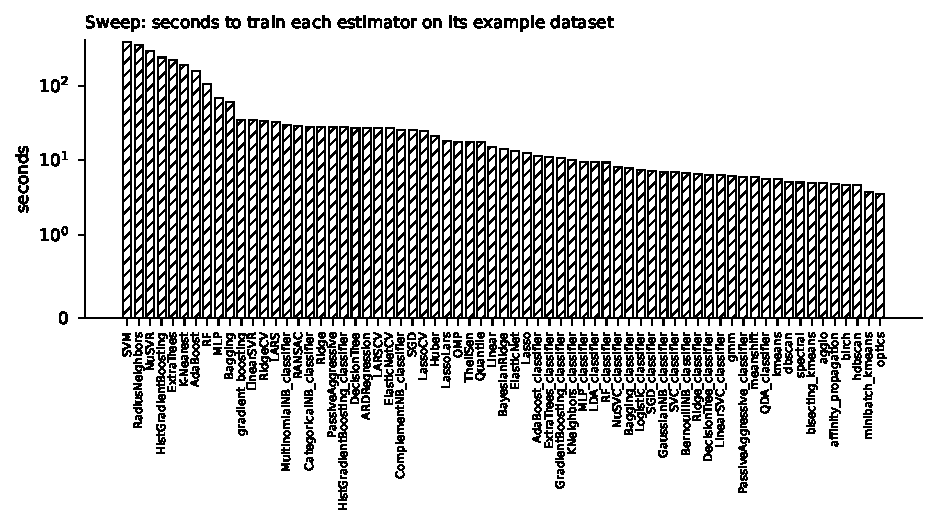
\includegraphics[width=\textwidth]{fig_sweep_seconds}
\caption{Seconds to train each of the 67 estimators in the sweep, symmetric log scale. Source: \code{every\_model\_sweep\_2026-09-24.json}.}
\label{fig:seconds}
\end{figure}

The round trip (\code{scripts/check\_artifact\_roundtrip.py}, record \code{docs/artifact\_roundtrip\_2026-09-24.json}) takes each of the 67 fitted estimators, writes it with skops 0.14.0 under the exact type allowlist, reads it back, and compares the predictions for the first eight rows of the dataset exactly, not within a tolerance. Sixty-six round-trip identically. \code{birch} cannot be written under the allowlist, and the application says so at export rather than writing an artifact that would need an unlisted type to load. The record stores the dataset hash, the seed, the artifact hash and both prediction vectors for every row, so a reader can rerun one estimator with \code{--only <model>} and compare against the stored numbers.

Together the two records bound the claim the paper makes about the registry. The application can train 67 estimators from its own form and can write and reload 66 of them; it does not claim that every hyperparameter of every estimator has been exercised, and the E1 finding on the nineteen classifiers (Section~\ref{sec:e1}) is the reason that claim is not made.
